\documentclass{article}
\usepackage{amsmath}
\usepackage{amssymb}
\usepackage{amsfonts}
\usepackage{graphicx}
\usepackage{mathrsfs}
\pagestyle{empty}
\usepackage[utf8]{inputenc}
\usepackage[T1]{fontenc}
\oddsidemargin 0.0in
\evensidemargin 0.0in
\textwidth 6.45in
\topmargin 0.0in
\headheight 0.0in
\headsep 0.0in
\textheight 9.0in

\usepackage{amsmath}\usepackage{tikz}
\usepackage{tkz-graph}
\usepackage{tkz-berge}
\usetikzlibrary{arrows,shapes}
\newcommand{\ZZ}{\Bold{Z}}
\newcommand{\NN}{\Bold{N}}
\newcommand{\RR}{\Bold{R}}
\newcommand{\CC}{\Bold{C}}
\newcommand{\QQ}{\Bold{Q}}
\newcommand{\QQbar}{\overline{\QQ}}
\newcommand{\GF}[1]{\Bold{F}_{#1}}
\newcommand{\Zp}[1]{\ZZ_{#1}}
\newcommand{\Qp}[1]{\QQ_{#1}}
\newcommand{\Zmod}[1]{\ZZ/#1\ZZ}
\newcommand{\CDF}{\Bold{C}}
\newcommand{\CIF}{\Bold{C}}
\newcommand{\CLF}{\Bold{C}}
\newcommand{\RDF}{\Bold{R}}
\newcommand{\RIF}{\Bold{I} \Bold{R}}
\newcommand{\RLF}{\Bold{R}}
\newcommand{\CFF}{\Bold{CFF}}
\newcommand{\Bold}[1]{\mathbf{#1}}

\begin{document}
\begin{center}{\Large\bf }\end{center}
\vspace{40mm}\[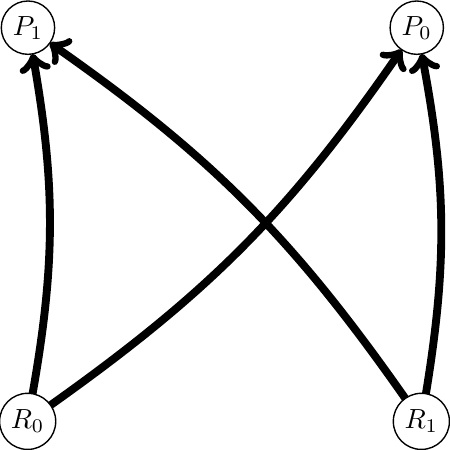
\begin{tikzpicture}
%
\useasboundingbox (0,0) rectangle (5.0cm,5.0cm);
%
\definecolor{cv0}{rgb}{0.0,0.0,0.0}
\definecolor{cfv0}{rgb}{1.0,1.0,1.0}
\definecolor{clv0}{rgb}{0.0,0.0,0.0}
\definecolor{cv1}{rgb}{0.0,0.0,0.0}
\definecolor{cfv1}{rgb}{1.0,1.0,1.0}
\definecolor{clv1}{rgb}{0.0,0.0,0.0}
\definecolor{cv2}{rgb}{0.0,0.0,0.0}
\definecolor{cfv2}{rgb}{1.0,1.0,1.0}
\definecolor{clv2}{rgb}{0.0,0.0,0.0}
\definecolor{cv3}{rgb}{0.0,0.0,0.0}
\definecolor{cfv3}{rgb}{1.0,1.0,1.0}
\definecolor{clv3}{rgb}{0.0,0.0,0.0}
\definecolor{cv0v1}{rgb}{0.0,0.0,0.0}
\definecolor{cv0v2}{rgb}{0.0,0.0,0.0}
\definecolor{cv3v1}{rgb}{0.0,0.0,0.0}
\definecolor{cv3v2}{rgb}{0.0,0.0,0.0}
%
\Vertex[style={minimum size=1.0cm,draw=cv0,fill=cfv0,text=clv0,shape=circle},LabelOut=false,L=\hbox{$R_{0}$},x=0.0cm,y=0.0cm]{v0}
\Vertex[style={minimum size=1.0cm,draw=cv1,fill=cfv1,text=clv1,shape=circle},LabelOut=false,L=\hbox{$P_{1}$},x=0.0038cm,y=5.0cm]{v1}
\Vertex[style={minimum size=1.0cm,draw=cv2,fill=cfv2,text=clv2,shape=circle},LabelOut=false,L=\hbox{$P_{0}$},x=4.9415cm,y=5.0cm]{v2}
\Vertex[style={minimum size=1.0cm,draw=cv3,fill=cfv3,text=clv3,shape=circle},LabelOut=false,L=\hbox{$R_{1}$},x=5.0cm,y=0.0cm]{v3}
%
\Edge[lw=0.1cm,style={->,bend right=10,color=cv0v1,},](v0)(v1)
\Edge[lw=0.1cm,style={->,bend right=10,color=cv0v2,},](v0)(v2)
\Edge[lw=0.1cm,style={->,bend right=10,color=cv3v1,},](v3)(v1)
\Edge[lw=0.1cm,style={->,bend right=10,color=cv3v2,},](v3)(v2)
%
\end{tikzpicture}\]
\end{document}